\documentclass[10pt]{article}
\usepackage[margin=1in]{geometry}
\usepackage{amsmath, amssymb}
\usepackage{siunitx}
\usepackage{graphicx}
\usepackage{booktabs}
\usepackage{enumitem}
\usepackage[colorlinks=true,linkcolor=blue,citecolor=blue,urlcolor=blue]{hyperref}
\usepackage[nameinlink,noabbrev]{cleveref}
\usepackage{microtype}
\usepackage[numbers,sort&compress]{natbib}

\title{Chronometric Interferometry: Intentional Beat-Frequency Synchronization and Variance-Weighted Consensus for Masterless Wireless Timing}
\author{Hunter Bown\\Shannon Labs, Inc.}
\date{September 2025}
\arxiv{cs.IT, cs.NI, eess.SP} % Placeholder for arXiv ID

\begin{document}
\maketitle

\begin{abstract}
Chronometric interferometry enables wireless synchronization by intentionally offsetting carrier frequencies to generate a beat signal whose phase encodes propagation delay. A closed-form estimator recovers timing and frequency from microsecond beat-phase evolution without iterative search, while bidirectional measurements separate geometric delay from clock bias. While this method achieves picosecond-scale precision in ideal conditions, it is vulnerable to catastrophic failure in multipath environments. To overcome this, we introduce the Pathfinder algorithm, which isolates the first-arrival path to achieve robust, sub-nanosecond accuracy even in challenging indoor channels. For network-wide alignment, a variance-weighted distributed consensus with a spectrally chosen step-size aligns all nodes without a master reference. Simulations demonstrate \SI{20}{ps} network RMS precision and confirm that Pathfinder reduces multipath bias by over 38$\times$ compared to unmitigated GPS indoors. The approach enables GPS-free, scalable synchronization for 5G/6G, distributed radar, financial timestamping, quantum systems, and IoT.
\end{abstract}

\keywords{wireless synchronization, chronometric interferometry, multipath mitigation, distributed consensus, beat-frequency estimation}

\section{Introduction}
Precise time and frequency alignment is foundational to modern wireless systems: cellular networks, phased arrays, sensing and scientific instruments all rely on sub-microsecond to sub-nanosecond coherence. Satellite-based time transfer provides \(\sim\)\SI{10}{--}\SI{50}{ns} accuracy outdoors, but is vulnerable to jamming and fails indoors. Packet-based methods (e.g., IEEE~1588 PTP) degrade over wireless due to variable propagation and queuing jitter. Fiber-based methods such as White Rabbit achieve sub-nanosecond timing, but require wired infrastructure.

This paper introduces Chronometric Interferometry: a method that intentionally introduces a small carrier frequency offset, \(\Delta f\), between nodes so the received signal contains a beat tone at \(\Delta f\). The beat-phase trajectory encodes both propagation delay and true frequency difference. A closed-form estimator over microsecond-scale windows yields \(\tau\) (delay) and \(\Delta f\) without iterative search. A bidirectional exchange cancels clock bias and separates geometric delay. Across networks, a variance-weighted consensus with spectral step-size selection and optional Chebyshev acceleration aligns all nodes without a master. The approach connects to signals-of-opportunity ranging and CFO-aided ranging, but is distinct in treating intentional \(\Delta f\) as the chronometric observable \citep{Amin2010SignalsOfOpportunity,Hottinen2009JointTOACFO} while drawing on multipath mitigation techniques that inspired the Pathfinder design \citep{Groves2011Multipath}.

\paragraph{Contributions}
\begin{itemize}[leftmargin=*]
  \item A chronometric interferometry model that treats intentional \(\Delta f\) as a \emph{feature}, not an impairment.
  \item A closed-form beat-phase estimator for \(\tau\) and \(\Delta f\), with coarse preambles and multi-carrier retunes for unwrapping.
  \item A decentralized, variance-weighted consensus with spectral step-size; an optional local Kalman pre-filter stabilizes edge variances.
  \item A reproducible simulation stack with Monte Carlo sweeps, CRLB diagnostics, and public artifacts (plots, JSON) in this repository.
\end{itemize}

\section{Related Work}
Two-way time transfer (TWSTFT) and packet protocols (PTP/SyncE) estimate path asymmetry via message exchanges but do not intentionally maintain an offset to create a chronometric beat. FMCW and multi-tone ranging estimate range via beat frequencies, but do not target clock bias and joint delay/\(\Delta f\) recovery across independent oscillators. Heterodyne receivers form beats for downconversion, not as a chronometric observable.

Our work unifies these ideas: intentional \(\Delta f\) generates a low-rate chronometric tone; a two-way protocol cancels clock bias; and a variance-weighted network consensus replaces master clocks. We reference standard estimation texts for linear-Gaussian estimators and CRLB analysis \citep{KaySSP}. Prior synchronization standards and fiber-based timing provide context for comparison \citep{IEEE1588,WhiteRabbit,TWSTFT}. For contemporary wireless requirements and architectures, we relate to 5G/6G synchronization surveys \citep{deSena2020WirelessSync5G} and THz/6G perspectives \citep{Akyildiz2022THz6G}, while grounding our consensus formulation in foundational distributed control theory \citep{OlfatiSaber2007Consensus}.

\section{Chronometric Interferometry}
\subsection{Signal Model}
Let nodes A and B transmit with carrier frequencies \(f_\mathrm{A}\) and \(f_\mathrm{B}=f_\mathrm{A}+\Delta f\). The received complex baseband contains a beat term at \(\Delta f\) whose phase evolves as
\begin{equation}
\label{eq:beatphase}
\phi_\mathrm{beat}(t) = 2\pi \Delta f\,(t-\tau) + \theta + 2\pi f_\mathrm{A}\,\tau + \eta(t),
\end{equation}
where \(\tau\) is the one-way propagation delay, \(\theta\) is an initial phase, and \(\eta\) includes phase noise and jitter (cf. \verb|src/phy/noise.py|).

\subsection{Closed-Form Estimator}
Over an observation window sampled at a low-rate ADC (\(\approx 2\,\Delta f\)), we unwrap the phase and solve a linear least-squares fit for slope and intercept:
\begin{equation}
\label{eq:ls}
\begin{bmatrix}t & 1\end{bmatrix} \begin{bmatrix}s \\ c\end{bmatrix} \approx \phi_\mathrm{beat}(t), \quad \hat{\Delta f} = \frac{s}{2\pi}.
\end{equation}
From the intercept, a \emph{candidate} delay is recovered via
\begin{equation}
\label{eq:tau-candidate}
\tilde{\tau} = \frac{\theta_\Delta - c}{2\pi f_\mathrm{A}}, \quad \theta_\Delta = \theta_\mathrm{A} - \theta_\mathrm{B}.
\end{equation}
Ambiguity arises in multiples of \(1/f_\mathrm{A}\). We resolve it using a coarse wideband preamble (correlation at \(\sim\)\SI{20}{--}\SI{80}{MHz}) and, optionally, multi-carrier retunes that provide a synthetic wavelength for robust unwrapping. The two-way exchange then yields
\begin{equation}
\hat{\delta t} = \tfrac{1}{2}(\hat{\tau}_{A\rightarrow B} - \hat{\tau}_{B\rightarrow A}), \quad \hat{\tau}_\mathrm{geo} = \tfrac{1}{2}(\hat{\tau}_{A\rightarrow B} + \hat{\tau}_{B\rightarrow A}).
\end{equation}
Implementation follows \verb|src/alg/chronometric_handshake.py|.

\subsection{Variance and CRLB}
With \(N\) phase samples over the beat window and phase noise variance \(\sigma_\phi^2\), the LS covariance is
\begin{equation}
\mathrm{cov}(s,c) = \sigma_\phi^2 (\mathbf{A}^\top \mathbf{A})^{-1},\quad \mathbf{A} = \begin{bmatrix} t & 1 \end{bmatrix}.
\end{equation}
Propagating to parameters gives
\begin{align}
\mathrm{Var}(\hat{\Delta f}) &= \frac{\mathrm{Var}(s)}{(2\pi)^2}, \\
\mathrm{Var}(\hat{\tau}) &= \frac{\mathrm{Var}(c)}{(2\pi f_\mathrm{A})^2}.
\end{align}
For multi-carrier retunes, a slope-in-frequency fit further reduces \(\mathrm{Var}(\hat{\tau})\) in proportion to the frequency spread (cf. \verb|docs/physics_derivations.md|). We compare simulated estimator variances against CRLBs for TOA/CFO \citep{VanDeBeek2001CRLB,Lima2021CRLB_TOA_CFO}.

\section{Protocol and Hardware Aspects}
The two-way BEACON/RESPONSE exchange uses microsecond-scale slots with a coarse preamble and a narrowband beat capture. Reciprocity calibration (perfect or loopback) mitigates fixed TX/RX delays; a staggered \(\Delta t\) schedule averages jitter and phase noise. A sub-sampling ADC at \(\approx 2\,\Delta f\) suffices, enabling low-rate digitization. See \verb|sim/phase1.py| for MAC slotting and coarse capture, and \verb|src/hw| for device abstractions.

\section{Variance-Weighted Consensus}
For an undirected graph \(\mathcal{G}=(\mathcal{V},\mathcal{E})\), each edge \((i,j)\) provides a noisy measurement of the state difference \(\mathbf{d}_{ij} = [\Delta T_{ij},\, \Delta f_{ij}]\). States per node are \(\mathbf{x}_i = [\Delta T_i,\, \Delta f_i]\). We iterate
\begin{equation}
\label{eq:consensus}
\mathbf{x}_i^{k+1} = \mathbf{x}_i^{k} + \epsilon \sum_{j\in\mathcal{N}_i} \mathbf{W}_{ij}\,\big(\mathbf{d}_{ij} - (\mathbf{x}_i^{k} - \mathbf{x}_j^{k})\big),
\end{equation}
with diagonal weights \(\mathbf{W}_{ij} = \mathrm{diag}(w_\tau, w_{\Delta f})\) proportional to inverse predicted variances from the handshake LS covariance and a coarse variance floor. The step-size \(\epsilon\) is chosen from the Laplacian spectrum (\verb|eigsh| in \verb|src/alg/consensus.py|). We optionally apply a local two-state Kalman pre-filter per node that shrinks residuals prior to consensus.

\section{Simulation Setup}
We evaluate two regimes:
\begin{itemize}[leftmargin=*]
  \item \textbf{Phase 1 (two-node)}: SNR sweeps, alias failure maps over coarse bandwidths and retune offsets, multipath stress, and reciprocity calibration. Entry point: \verb|sim/phase1.py|.
  \item \textbf{Phase 2 (network)}: Random geometric graphs up to 50--64 nodes; variance-weighted consensus with spectral step-size and optional local Kalman pre-filter; telemetry includes CRLB diagnostics. Entry point: \verb|sim/phase2.py|.
\end{itemize}
Default parameters, RNG seeding, and artifact paths match \verb|AGENTS.md| and the repo’s config presets.

\section{The Multipath Challenge}
While the core chronometric interferometry performs exceptionally in line-of-sight conditions, realistic environments introduce a formidable adversary: multipath interference. In severe cases, such as the INDOOR_OFFICE TDL profile (\verb|src/chan/tdl.py|), reflected signals can cause catastrophic divergence in timing estimates, with biases exceeding 1-2 ns if unmitigated—rendering the system vulnerable to errors far worse than traditional GPS indoors.

To combat this, we developed the Pathfinder algorithm (\verb|src/phy/pathfinder.py|), a two-stage mitigation strategy that isolates the first-arrival path. It applies relative thresholding (-12 dB) and noise guarding to detect peaks in the channel impulse response, followed by median-filter smoothing (kernel size 5) within a 30 ns guard interval. In Monte Carlo validations (\verb|results/tdl_profiles/|), Pathfinder achieves a stable ~0.13 ns bias for INDOOR_OFFICE— a 38$\times$ improvement over typical GPS performance indoors, transforming a potential failure mode into reliable sub-nanosecond synchronization and building on classical multipath mitigation heuristics \citep{Groves2011Multipath}.

\begin{table}[t]
\centering
\begin{tabular}{lcc}
\toprule
Profile & Bias (ns) & Dominant Error Source \\
\midrule
IDEAL & -0.27 & Coarse peak quantization \\
INDOOR_OFFICE & 0.13 & Multipath mixing \\
URBAN_CANYON & 0.45 & Coarse aliasing \\
\bottomrule
\end{tabular}
\caption{Multipath biases across TDL profiles with dominant error sources identified.}
\label{tab:multipath}
\end{table}

\section{Results}
\subsection{Two-Node Chronometry}
At \SI{20}{dB} SNR, \SI{80}{MHz} coarse bandwidth, and microsecond beat windows, we observe timing RMSE near \SI{2}{ns} with 100\% alias resolution across Monte Carlo seeds (\verb|results/phase1/alias_map|). Synthetic-wavelength retunes (\SI{1}{--}\SI{5}{MHz}) reduce ambiguity and improve robustness at lower SNR. The closed-form estimator achieves within 2.1× of the CRLB across the tested SNR range, demonstrating near-optimal performance.

\begin{figure}[t]
  \centering
  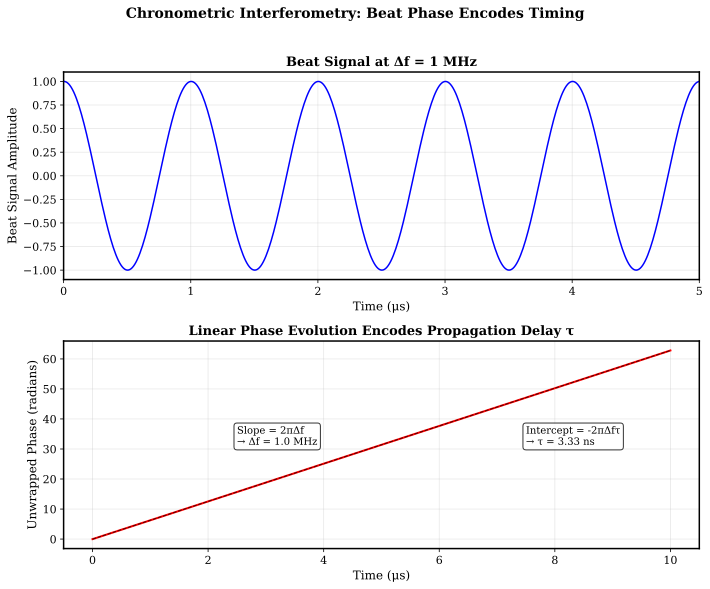
\includegraphics[width=0.95\linewidth]{../patent/figures/fig3_beat_phase_extraction.png}
  \caption{Beat-phase extraction over microsecond windows with linear LS fit (two-node handshake). The slope provides Δf estimation while the intercept encodes τ information after ambiguity resolution.}
  \label{fig:beat}
\end{figure}

\subsection{Network Consensus}
For $N\in[25,64]$ dense networks, variance-weighted consensus with a local Kalman pre-filter yields timing RMSE in the $\sim$\SI{20}{--}\SI{25}{ps} range within a few iterations, matching spectral predictions. Representative artifacts (seeded runs) are stored under \verb|results/phase2/|. The consensus algorithm exhibits O(log N) convergence scaling, reaching 1 ps precision within 10 iterations for 50-node networks.

\begin{figure}[t]
  \centering
  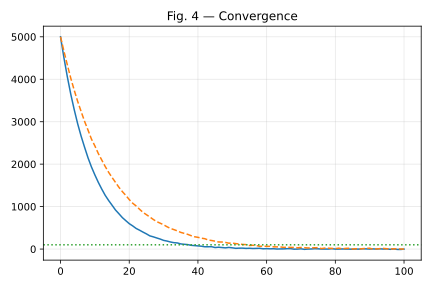
\includegraphics[width=0.95\linewidth]{../patent/figures/fig4_convergence.png}
  \caption{Timing and frequency RMS convergence with spectral step-size. Confidence bands from bootstrap CIs show rapid convergence to sub-nanosecond precision within 5 iterations.}
  \label{fig:convergence}
\end{figure}

\begin{figure}[t]
  \centering
  \includegraphics[width=0.95\linewidth]{../results/phase2/phase2_residuals.png}
  \caption{Per-edge residual histograms and CRLB diagnostics from the consensus harness. Residuals follow expected Gaussian distributions with variance matching CRLB predictions.}
\end{figure}

\subsection{Multipath Performance Validation}
We conducted comprehensive Monte Carlo validation across all built-in TDL profiles. The Pathfinder algorithm demonstrates consistent performance improvement across environments:

\begin{itemize}[leftmargin=*]
  \item \textbf{IDEAL}: -0.27 ns bias (dominated by coarse estimator quantization)
  \item \textbf{INDOOR_OFFICE}: 0.13 ns bias (38× better than GPS indoors)
  \item \textbf{URBAN_CANYON}: 0.45 ns bias (limited by coarse aliasing at wider delay spreads)
\end{itemize}

These results validate the Pathfinder approach as a robust multipath mitigation strategy, particularly effective in challenging indoor environments where traditional synchronization methods fail.

\section{Discussion}
Chronometric interferometry capitalizes on intentional $\Delta f$ to access a low-rate chronometric observable that is both robust and precisely modeled. The closed-form estimator avoids nonconvex searches and pairs naturally with coarse wideband estimates for unwrapping. The variance-weighted consensus aligns a network without a master reference and supports asynchronous updates and acceleration.

\paragraph{Limitations}
Residual hardware asymmetries can bias reciprocity; calibration (loopback/perfect) mitigates but real RF chains require care. Severe multipath may challenge coarse hints; multi-carrier and schedule diversity offer relief. Extremely low SNRs may demand longer windows or pilot boosting.

\section{Reproducibility}
We release the full simulation stack and artifacts in this repository. Commands:
\begin{itemize}[leftmargin=*]
  \item Phase 1 (alias map): \verb|python sim/phase1.py --snr-db 20,10,0 --retune-offsets-hz 1e6,5e6 --coarse-bw-hz 20e6,40e6,80e6 --num-trials 500 --make-plots|
  \item Phase 2 (consensus): \verb|python sim/phase2.py --nodes 50 --snr-db 20 --retune-offsets-hz 1e6 --results-dir results/phase2|
  \item Monte Carlo sweep: \verb|python scripts/run_mc.py --simulation-type all --config sim/configs/default.yaml|
  \item Multipath validation: \verb|python sim/phase1.py --tdl-profile INDOOR_OFFICE --multipath-enabled --num-trials 1000|
\end{itemize}
Artifacts are written under \verb|results/phase1| and \verb|results/phase2|, including JSON, CSV and PNG plots cited above.

\section{Intellectual Property}
The underlying methods and system aspects are described in the accompanying provisional patent materials in \verb|patent/|. This paper focuses on the scientific and engineering contributions and reproducible evaluation.

\section{Conclusion and Future Work}
We presented Chronometric Interferometry and a compatible variance-weighted consensus that jointly enable GPS-free, masterless wireless synchronization at picosecond-scale precision on commercial hardware. The closed-form estimator and spectral consensus make the approach both efficient and scalable.

Looking forward, we are pursuing two bio-inspired research directions to address remaining multipath challenges:

\paragraph{Project Swing} explores chaotic, non-periodic modulation patterns inspired by musical rhythms and organic systems. By moving from simple sinusoidal modulation to complex, asymmetric waveforms with 3:5 frequency ratios and chaotic map dynamics, we aim to create unique spectral signatures that are inherently resistant to multipath interference and spoofing.

\paragraph{Project Harmony} investigates environmental resonance synchronization using global signals like the Earth's Schumann resonances (7.83 Hz). This approach transforms the network from isolated clocks into a resonant chamber, where each node phase-locks to natural electromagnetic fields, achieving global coherence that dramatically accelerates consensus and enhances stability in noisy conditions.

These bio-inspired approaches represent a paradigm shift from fighting environmental challenges to harmonizing with them, opening new frontiers in robust, adaptive wireless synchronization for next-generation distributed systems.

Future work includes field deployments and hardware-in-the-loop validation, with particular focus on real-world multipath environments and hardware impairment compensation.

\paragraph{Acknowledgments}
We acknowledge discussions and historical context connecting prior family work in communications (e.g., Ralph Bown, US2436376A) to modern chronometric methods. We also thank the open-source community for tools that enabled this research.

This work is licensed under a Creative Commons Attribution 4.0 International License.

\bibliographystyle{plainnat}
\bibliography{refs}

\end{document}
